\input{thesis_header.tex}

% \usepackage{cite}
\usepackage{amsmath,amssymb,amsfonts}
\usepackage{algorithmic}
\usepackage{graphicx}
\usepackage{textcomp}
\usepackage{xcolor}

% Table stuff
% \usepackage{booktabs}
\usepackage{multirow}
\usepackage{longtable}

% Figure stuff
\usepackage{tikz}
\usepackage{fancyvrb}

% Bibliography
\bibliographystyle{IEEEtran}
% \addbibresource{references.bib}

\begin{document}

% This is the table of contents, list of figures, list of tables, formatted correctly.
% romanpages ~ pages numbered by roman numerals
\begin{romanpages}
    \maketitle
    \begin{abstract}

Decompilation is the process of reverse engineering a binary program into an equivalent source code representation with the objective to recover high-level program constructs such as functions, variables, data types, and control flow mechanisms. Decompilation is applicable in many contexts, particularly for security analysts attempting to decipher the construction and behavior of malware samples. However, due to the loss of information during compilation, this process is naturally speculative and thus is prone to inaccuracy. This inherent speculation motivates the idea of an evaluation framework for decompilers.

In this work, we present a novel framework to quantitatively evaluate the inference accuracy of decompilers, regarding functions, variables, and data types. Within our framework, we develop a domain-specific language (DSL) for representing such program information from any "ground truth" or decompiler source. Using our DSL, we implement a strategy for comparing ground truth and decompiler representations of the same program. Subsequently, we extract and present insightful metrics illustrating the accuracy of decompiler inference regarding functions, variables, and data types, over a given set of benchmark programs. We leverage our framework to assess the correctness of the Ghidra decompiler when compared to ground truth information scraped from DWARF debugging information. We perform this assessment over a subset of the GNU Core Utilities (Coreutils) programs and discuss our findings.
        
    \end{abstract}
    \begin{acknowledgements}

The pursuit of my master's degree wouldn't have been possible without the tremendous support of many amazing people. First, I want to thank my advisor, Dr. Prasad Kulkarni, for providing me with a special research opportunity and for supporting me on my research journey. I am also grateful for the reception of the NSF Cybercorps Scholarship for Service (SFS), made possible by Dr. Bo Luo and several others. Next, I want to thank my friends and peers for providing fantastic academic and emotional support throughout the entirety of my undergraduate and graduate studies. Lastly, I want to thank my entire family - particularly my father, Aaron Kline, and my two sisters, Jenna and Julia Kline - for their endless love and support. I also want to honor my late mother, Beth Kline, for the amazing person she was and the continued impact she has on me.
                
    \end{acknowledgements}
    \tableofcontents{}
    \listoffigures
    \listoftables
\end{romanpages}

\chapter{Introduction} \label{sec:introduction}

\section{Context and Background}

In an increasingly digital world, cybersecurity has emerged as a crucial consideration for individuals, companies, and governments trying to protect their information, financial assets, and intellectual property. Of the many digital threats, various forms of malware continue to pervade the digital landscape and thus remain a key concern for security analysts. One approach to combating malware is to deconstruct and reason about the malware itself. Understanding the functionality and behavior of malware samples may aid a security analyst in identifying methods to thwart or disable the malware's effects on a target system and similar systems.

Although simple in concept, the act of reverse engineering and reasoning about malware proves to be a steep challenge. The primary issue is that access to high-level malware source code is almost never available and, thus, any reasoning about the malware must be derived from the malware binary. Another issue is that malware authors often leverage obfuscation techniques to mask the intention and behavior of malware samples. To evade antivirus tools using signature-based detection, malware authors may employ techniques such as dead-code insertion, register reassignment, subroutine reordering, instruction substitution, code transposition, and code integration \cite{bib:malware-obfuscation-techniques}. To complicate semantic binary code analysis of malware samples, malware authors may leverage compile-time strategies such as stripping and compiler optimizations \cite{bib:practical-analysis-stripped-binary-code}. Along with the employment of these obfuscation strategies in the context of malware, these techniques may be also leveraged by developers or companies to dissuade binary code analysis of proprietary software.

Despite the challenge of binary code analysis, there exist many tools that attempt to glean high-level semantic information from binary code samples. A \emph{disassembler} takes binary code as input and produces assembly code as output. Many challenges and considerations exist in the disassembly process, particularly for stripped binary code, such as discerning code from data and locating function boundaries \cite{bib:disassembly-challenges}. One invariant in the disassembly process, however, is that the mapping from assembly instructions to binary instructions and vice-versa is always one-to-one. A \emph{decompiler} takes this reverse mapping process one step further by translating binary code into an equivalent high-level source code representation. The decompilation process is inherently speculative since high-level information such as function boundaries, variables, data types, and high-level control flow mechanisms are lost when a program is compiled. With this, the decompiler must infer enough high-level structure for useful analysis without being overly aggressive and consequently blurring the program's intent. Many decompiler tools are currently in use by the reverse engineering community. Commercial decompiler tools include IDA Pro \cite{bib:ida} and JEB3 \cite{bib:jeb}. Popular open-source decompiler frameworks include Ghidra \cite{bib:ghidra} and RetDec \cite{bib:retdec}.

\section{Research Problem}

Due to the proposed utility of decompiler tools as well as the imprecise nature of decompilation, a generalized and extensible quantitative evaluation framework for decompilers is critical. Existing work by Liu et. al \cite{bib:how-far-weve-come} proposes an evaluation technique to determine whether recompiled decompiled programs are consistent in behavior to their original binaries. Work by Naeem et. al \cite{bib:metrics-effectiveness-decompilers} proposes a set of metrics for assessing the clarity of decompiled Java programs with respect to program size, conditional complexity, identifier complexity, number of local variables, and expression complexity. These works, although insightful for assessing decompiler quality, do not measure the recovery accuracy of high-level program constructs such as functions, variables, and data types. The recovery and inference of the these high-level constructs, in conjunction with clarity and behavioral correctness, is important for analysts to gain an understanding of decompiled binary programs.

\section{Research Objectives}

Targeting the current gap in the literature outlined in the previous section, this paper presents a novel framework for quantifying and assessing the accuracy of decompiler tools with respect to high-level program constructs, including functions, variables, and data types. To prove our concept, we apply our framework to the Ghidra decompiler and discuss our findings. The primary objectives achieved by this work are as follows:

\begin{enumerate}
    \item We define a domain-specific language (DSL), written in Python, for expressing high-level program information including functions, variables, and data types. This serves as a medium whereby we can translate program information extracted from a decompiler or a ground-truth source.
    \item We extend our DSL to compare program information representations from different sources. The primary use case is to compare ground-truth program information to decompiler-inferred program information.
    \item Leveraging the comparison logic in (2), we define a set of quantitative metrics to measure the accuracy of function, variable, and data type inference.
    \item We develop a translation module in Python that uses DWARF debugging information from a binary program to generate a ground-truth program information representation in our DSL.
    \item We utilize the Ghidra Python API to implement a translation module. This module takes Ghidra decompilation of a binary program as input and outputs a program information representation in our DSL.
    \item Using our developed language, metrics, and translation modules, we quantitatively assess the accuracy of the Ghidra decompiler when compared to ground truth program information obtained from DWARF debugging information. We peform this analysis using the set of GNU Coreutils programs as benchmarks. We present the evaluation results and discuss additional findings and takeaways.
\end{enumerate}

\section{Evaluation Summary}

We use our evaluation framework to perform an assessment of the Ghidra decompiler (version 10.2) over 105 GNU Core Utilities (version 9.1) benchmark programs compiled with GCC (version 11.1.0). We evaluate Ghidra with no optimizations under three compilation cases of the benchmark programs - (1) stripped, (2) standard (not stripped, no DWARF symbols added), and (3) debug (DWARF symbols included) - to determine how the type and quantity of information provided in the binaries affects recovery and inference performance of functions, variables, and data types by Ghidra.

Our function recovery analysis reveals that Ghidra successfully recovers 100\% of the 18139 functions under the stripped and standard compilation conditions across all benchmarks. In the debug compilation case, Ghidra successfully identifies all functions but fails to decompile four functions in the \emph{factor} program due to a type resolution error. Upon further analysis, we conclude this is a bug in the Ghidra decompiler.

Analysis of high-level variable recovery shows that the recovery accuracy of variables of primitive data types (char, int, float, pointer) is significantly higher than the recovery accuracy of complex (aggregate) types (array, struct, union), particularly in the stripped and standard compilation cases when no debugging information is present. Overall, we see a partial high-level variable recoveries percentages of 97.1\%, 99.2\%, and 99.9\% for the three compilation cases, respectively. The percentages of exact high-level variable matches for each of the compilation cases are 36.1\%, 38.6\%, and 99.6\%, respectively.

Related to our high-level variable recovery analysis, we perform a "decomposed" variable recovery analysis. For the decomposition, we recursively decompose each variable into a set of primitive variables as they appear in memory. We then perform the comparison and evaluation similar to in the high-level analysis. We show that the partial recovery percentages for each of the stripped, standard, and debug compilation cases are 73.8\%, 92.4\%, and 98.0\%, respectively. The exact match percentages over the decomposed variables are 24.6\%, 25.0\%, and 98.0\% for each of the compilation cases, respectively. The lower recovery accuracy results in this decomposed analysis are explained by the decomposition of the variables with complex types, namely arrays, that are partially or fully missed in the high-level analysis. These variables, when decomposed, result in an increase in the number of total missed variables. Analysis of decomposed variable recovery by data type shows that int (and char) variables are most accurately inferred, followed by pointer variables, with floating-point (float, double) variables showing the lowest recovery accuracy.

We perform a data bytes recovery analysis to determine the total percentage of data bytes that are found and missed across all ground truth variables by the decompiler. We discover that the bytes recovery percentages are 61.3\%, 80.6\%, and 99.5\% for each the stripped, standard, and debug compilation cases, respectively.

Lastly, we perform an evaluation of the Ghidra decompiler's array recovery accuracy. We find that, for each the stripped, standard, and debug compilation cases, 36.2\%, 71.6\%, and 99.5\% of ground truth array varnodes overlap with at least one associated decompiler-inferred array varnode, respectively. We find the average size (in bytes) discrepancies between compared ground truth and the decompiler variables to be 458.6, 239.0, and 9.42 for each of the compilation cases, respectively. When scaled with respect to the sizes of the ground truth arrays, the average array size error percentages for the array comparisons in each compilation case are 91.2\%, 47.5\%, and 11.0\%, respectively.

Across our analyses, we observe that there is a clear relationship between the compilation configuration of the benchmark programs and the recovery accuracy of program constructs by the Ghidra decompiler. We find that, with respect to recovery of program constructs, the debug compilation case far outperforms the standard case, which moderately outperforms the stripped case. However, despite the relatively high recovery accuracy of the Ghidra decompiler in the debug case, we futher explore the causes of misses and partial misses in the debug case and find that Ghidra possesses a major limitation in expressing local variables declared in lexical scopes below the top level of a function. A compiler such as GCC may reuse stack address space for variables associated with disjoint (non-overlapping and non-nested) lexical scopes. This is a problem for the Ghidra decompiler as we observe that all variable declarations are placed at the top level of the function, ultimately preventing these scope-specific variables from being precisely captured. From our manual analysis of the decompiled benchmark programs, we find that this is the cause of the majority of partially missed variables and data bytes in the debug compilation case. This limitation affects the stripped and standard compilation cases as well.

\section{Contributions}

The three key contributions of this work are as follows:
\begin{enumerate}
    \item We develop a novel framework for evaluating decompiler tools based on the recovery accuracy of high-level program constructs, including functions, variables, and data types. This framework includes a domain-specific language (DSL), developed in Python, to represent and compare sources of high-level program information and their association with binary-level information. In addition, we devise quantitative metrics for expressing the recovery accuracy of high-level program constructs.
    \item We leverage our framework to perform an in-depth evaluation of the Ghidra decompiler with respect to high-level function, variable, and data type recovery. This evaluation is performed over the GNU Core Utilities programs under three compilation conditions.
    \item From our evalution of Ghidra, we discover and discuss the implications of two key issues present in the Ghidra decompiler.
\end{enumerate}

\section{Outline}

The remainder of this paper is outlined as follows: In Chapter \ref{sec:background-related-work}, we discuss related research and background concepts useful for the understanding of this work. Next, in Chapter \ref{sec:methodology}, we detail our methodology for developing our evaluation framework. In Chapter \ref{sec:evaluation}, we present and discuss the results of applying our evaluation framework to the Ghidra decompiler. We conclude in Chapter \ref{sec:conclusion} with a summary of our results, implications of our work, limitations, and future research directions.

\chapter{Background and Related Work} \label{sec:background-related-work}

\section{Software Reverse Engineering, Dissassembly, and Decompilation}

\emph{Software reverse engineering (SRE)} is the process of analyzing a software system with the intention to extract design and implementation information, particularly in situations where high-level source code is unavailable \cite{bib:sre}. One common use case for this practice is to understand and deconstruct legacy code present in a software system where the source code has been lost. In this scenario, analysts could use SRE to understand this legacy code, determine its behavior, and ultimately decide how to reuse, patch, or replace the code. Another context for the use of SRE is computer security. Malware, or malicious programs, are nearly always encountered in binary form without their associated high-level source code. An analyst may use SRE to deconstruct the malware's logic, determine its behavior, and identify approaches to neutralize the malware and harden the host system for prevention of future attacks.

To perform SRE on a binary program, a critical first step is \emph{disassembly}. This process takes binary code as input and produces assembly code as output. A key to this process is that binary and assembly instructions are always mapped one-to-one, and thus the main challenges lie in determining function boundaries and differentiating code, data, and metadata. Factors that contribute to these challenges include the following \cite{bib:disassembly-challenges}:
\begin{itemize}
    \item Data embedded in code regions
    \item Variable instruction size (on some architectures)
    \item Indirect branch instructions (the target of a branch instruction is not statically known)
    \item Functions without explicit `CALL` references
    \item Position independent code sequences
    \item Manually crafted assembly code
\end{itemize}

The conversion of binary code to assembly code through disassembly is a desirable starting point in the process of SRE. However, program semantics are still often difficult to interpret and reason about at the assembly code level. This difficulty necessitates an even more speculative process, \emph{decompilation}, that takes a binary program as input and produces a high-level source code representation of the input program's semantics, usually in C. Decompilation, therefore, involves the speculative inference of high-level constructs such as control flow mechanisms, variables, and data types. Decompiler tools rely heavily on the disassembly process as a first step in their analysis, and therefore the challenges affecting disassembly also naturally affect decompilation. Additional factors that obfuscate the accuracy of decompilation are the following:
\begin{itemize}
    \item Compiler optimizations
    \item Stripped debugging information and metadata
\end{itemize}

With these compounding challenges affecting the decompilation process, it is clear that decompiler tools operate under a great degree of uncertainty and speculation. This fact highlights the need for a common evaluation framework for decompiler tools.

\section{DWARF Debugging Standard}

\emph{DWARF} \cite{bib:dwarf} is a debugging file format used by many compilers and debuggers to support source-level debugging for compiled binary programs. When specified flags (usually '-g') are present at compilation, DWARF-supporting compilers such as GCC and Clang will augment the outputted binary program or object file with DWARF debugging information. A resulting binary executable can then be loaded into a DWARF-supporting debugger such as GDB to debug the target binary program with references to line numbers, functions, variables, and types in the source-level program. The DWARF standard is source language agnostic, but generally supports equivalent representations for constructs present in common procedural languages such as C, C++, and Fortran. In addition, DWARF is decoupled from any architecture or operating system. The generalizability of DWARF debugging information makes it a prime candidate for extracting "ground truth" information about a particular binary program, regardless of the specifics of the source language, architecture, or operating system. DWARF is leveraged in this work to scrape ground-truth information about target binary programs. This information is subsequently used to evaluate the accuracy of the output produced by a target decompiler.

\section{Ghidra Reverse Engineering Framework}

\emph{Ghidra} \cite{bib:ghidra}, created and maintained by the National Security Agency (NSA) Research Directorate, is an extensible software reverse engineering framework that features a disassembler, decompiler, and an integrated scripting environment in both Python and Java. We use the Ghidra decompiler in this work to demonstrate our decompiler evaluation framework.

\section{Related Work}

In the 2020 paper \emph{How Far We Have Come: Testing Decompilation Correctness of C Decompilers} by Liu et. al \cite{bib:how-far-weve-come}, the authors present an approach to determine the correctness of decompilers outputting C source code. They aim to find decompilation errors, recompilation errors, and behavior discrepancies exhibited by decompilers. To evaluate behavioral correctness, they attempt to recompile decompiled binaries (after potential syntax modifications) and use existing dynamic analysis techniques such as fuzzing to find differences in behavior between the recompiled and original programs. The objective of our work differs as we aim to evaluate decompiler inference of high-level structures such as functions, variables, and data types. Accurate inference of high-level structures enables easier understanding of decompiled programs by analysts; however, accurate behavior is also necessary to ensure that the decompiled representation is consistent with the original program. Hence, both of these works evaluate important aspects of decompiler correctness.

The review \emph{Type Inference on Executables} by Caballero and Lin \cite{bib:type-inference-executables} provides a comprehensive summary of recent literature on techniques used for variable discovery and type inference. In addition, the authors present various software reverse engineering (SRE) tools and frameworks in terms of their inputs, analysis types, output formats, and use cases. In essence, this work surveys the a set of decompiler tools and characterizes them based on their purported capabilities. The purpose of our work, on the contrary, is to objectively determine the correctness of decompiler tools based on their inference accuracy of high-level program constructs.

The 2006 technical report by Naeem et. al \cite{bib:metrics-effectiveness-decompilers} proposes a set of metrics for assessing the "cognitive expressibility" (clarity) of decompiled Java code. This is achieved through metrics that capture program size, conditional complexity, identifier complexity, number of local variables, and expression complexity. Despite the importance of these aspects in assessing the quality of a decompiler, this approach does not consider the "correctness" - either behavioral or structural - of the decompiled code. In addition, this work only targets decompiled Java programs.

Several existing works propose methodologies and frameworks targeting high-level variable and type inference from binary programs \cite{bib:divine, bib:tie, bib:artiste, bib:rewards, bib:scalable-variable-datatype-detection, bib:retypd}. Many of these works contain an evaluation of their inference accuracy; however, none of these works demonstrate evaluation metrics that express a unified assessment of function, variable, and data type recovery. Our work aims to fill this gap by providing a common and reusable framework for the recovery assessment of these high-level constructs, decoupled from the source of the extracted program information.

\chapter{Methodology} \label{sec:methodology}

In this section, we discuss the design, construction, and evolution of our decompiler evaluation framework. To achieve this, we identify key objectives that we subsequently address in more detail in the following sections. These objectives are as follows:

\begin{enumerate}
    \item Express program information such as functions, variables, data types, and addresses in a common language.
    \item Programmatically capture a "ground truth" representation of program information for a given binary program.
    \item Programmatically scrape program information from decompiler tools, namely Ghidra.
    \item Compare two program representations of the same program expressed in our common language.
    \item Formulate quantitative metrics for evaluating the accuracy of a decompiler.
\end{enumerate}

\section{Domain-Specific Language (DSL) for Program Information}

In order to make our framework general and reusable, we devise a common domain-specific language (DSL) to represent program information such as functions, variables, data types, and addresses, as well as the relationships between them. This DSL must act as a bridge linking binary-level address information with the source-level structures such as functions, variables, and data types. Combining the information from these two layers of abstraction is, in essence, a mapping between binary-level and source-level structures. The accuracy of this mapping for a given decompiler is precisely the objective of our analysis.

% [Figure representing how DSL can be constructed from many sources (DWARF, Ghidra, IDA Pro, etc.)]
\begin{figure}
    \centering
    \scalebox{0.8}{
        \input{./figures/proginfo-sources.latex}
    }
    \caption{DSL \emph{ProgramInfo} extraction from multiple sources}
    \label{fig:proginfo-sources}
\end{figure}

The DSL we devised is entirely decoupled from the source of the program information. This allows any ground truth or decompiler source of program information to be translated into this common language and subsequently analyzed or compared with another source of program information. The core of our language is defined in Python and is compatible with Python (Jython or CPython) versions >= 2.7. We chose Python because the Ghidra framework supports custom Python scripts for querying and manipulating program information obtained from the disassembler and decompiler. In addition, the Python 'pyelftools' open-source library \cite{bib:pyelftools} allows scraping DWARF debugging information directly from binary programs. This DWARF information can then be utilized to construct a "ground truth" representation of program information. We discuss this further in the next subsection.

\subsection{DSL Definitions}

\begin{figure}
    \centering
    \scalebox{0.4}{
        \input{./figures/dsl.latex}
    }
    \caption{Simplified DSL class relationships}
    \label{fig:dsl}
\end{figure}

In this section, we briefly describe the structure and relationships of the major constructs that comprise our DSL.

At the root of our DSL is the \emph{ProgramInfo} type. The fields of this type include a list of global variables (\emph{Variable} objects) and a list of functions (\emph{Function} objects).

The \emph{Function} type holds information about a function such as the name, the start PC address (\emph{Address} object), the end PC address (\emph{Address} object), a list of parameters (\emph{Variable} objects), a list of local non-parameter variables (\emph{Variable} objects), and the return type (\emph{DataType} object).

The \emph{Variable} type contains information about a source-level global variable, local variable, or parameter. A variable has a name, a data type (\emph{DataType} object), and a list of address "live ranges". We consider an address live range (\emph{AddressLiveRange} type) to be the association of a variable's storage address with the PC address range where the storage location is valid for the variable. This "live range" concept allows for the expression of source-level variables that map to multiple underlying storage locations throughout their lifetime. Multiple live ranges may be associated with a single variable when compiler optimizations are present.

The \emph{Address} type represents any absolute or relative location referenced in a binary program. This could include a PC location, variable storage location, or a register. From an implementation perspective, \emph{Address} is the base class with subclasses representing the different types of address constructions based on context. These \emph{Address} subclasses include \emph{AbsoluteAddress}, \emph{RegisterAddress}, \emph{RegisterOffsetAddress}, and \emph{StackAddress}. Each address is associated with an \emph{AddressRegion}. This type is used to manage ordering and comparison logic for addresses that fall within the same region.

The last main construct in our core DSL is \emph{DataType}. This type is represents a source-level data type and is typically associated with a variable or a function return type. \emph{DataType} is the base of a class hierarchy with subclasses representing particular data types. The subclasses include \emph{DataTypeFunctionPrototype}, \emph{DataTypeInt}, \emph{DataTypeFloat}, \emph{DataTypeUndefined}, \emph{DataTypeVoid}, \emph{DataTypePointer}, \emph{DataTypeArray}, \emph{DataTypeStruct}, \emph{DataTypeUnion}. Although these defined types correspond to C-like data types, this language can easily be extended to support other data types present in other high-level programming languages. All data type objects contain a "size" field representing the number of bytes the given data type occupies in memory.

\section{Capturing Ground Truth Program Information}

With our DSL defined, we need a reliable method to extract "ground truth" information from a program and translate this information into our DSL. This "ground truth" information is intended to be used in a comparison with the program information obtained from a decompiler. Our framework is meant for evaluation and therefore we assume that we have access to the source code of benchmark programs to be used for the evaluation. With this assumption, we consider two options for extracting program information from a given source program.

The first option for extracting ground truth information is to parse the source code's abstract syntax tree (AST) and then use this AST to manually extract functions, variables, and data types. There are two major issues with this approach. First, parsing source code to an AST assumes a particular source programming language which greatly reduces generality. Second, obtaining the AST alone does not offer any binary-level information that allows us to link binary-level addresses with the source-level structures.

The second, more favorable, approach to extracting ground truth program information involves leveraging debugging information optionally included in the binary by the compiler. The primary purpose of debugging information is to link binary-level instructions and addresses with source-level structures. This binary-level to source-level association is precisely what is needed to translate program information into our DSL. We choose the DWARF debugging standard as the assumed debugging format for our framework. However, defining a translation module from another debugging format into our DSL is certainly possible and is an idea for future work. The DWARF debugging standard is supported by nearly all major Linux compilers and may be extended to support any source-level programming language. These properties of the DWARF standard allow it to be used as a "ground truth" source of program information, decoupled from the source language or the compiler.

\subsection{Translating DWARF to the DSL}

Starting with a source-level program, we must perform the following steps to extract program information represented in our DSL. First, we compile the source program with the option to include debugging symbols. In our particular analysis we use the GCC compiler specifying the "-g" flag. Many other compilers also offer the option for compilation with the inclusion of DWARF debugging symbols. After we compile the program, we then extract the DWARF debugging information from the resulting binary. We utilize the 'pyelftools' Python library \cite{bib:pyelftools} to perform this extraction. The extraction results in, among other information, a set of debugging information entries (DIEs). Together, these DIE records provide a description of source-level entities such as functions, variables, and data types in relation to low-level binary information such as PC addresses and storage locations. Each DIE contains the following important features:

\begin{itemize}
    \item An \emph{offset} uniquely identifying the DIE within its compilation unit. These offsets are how DIEs reference other DIEs.
    \item A \emph{tag} representing the "class" of the DIE. Example tags include "DW\_TAG\_subprogram", "DW\_TAG\_variable", and "DW\_TAG\_base\_type".
    \item A set of \emph{attributes} specifying tag-specific properties of the DIE. Examples include "DW\_AT\_name", "DW\_AT\_size", and "DW\_AT\_type".
\end{itemize}

The translation process from the DIE graph into our DSL is, at its core, a process of forming a nested data structure (our DSL's \emph{ProgramInfo} type) from a flattened one (a collection of DWARF DIEs). To tackle this translation, we first define an intermediate representation (IR) language that acts as a "flattened" analog to the constructs present in our DSL. Instead of each IR construct directly containing the fields of other constructs, they instead contain fields that reference the IDs of other constructs through a shared database. The responsibility of the database is to map unique IDs to the flattened constructs. When all the IR constructs have been inserted into the database, we use the database to recursively resolve the flattened IR structures into their associated DSL structures, starting from the root \emph{ProgramInfoStub} object, the IR analog to the \emph{ProgramInfo} DSL type. This process is complicated by the fact that some data types, particularly \emph{struct} types, may be recursive or mutually recursive, ultimately creating a cycle in the reference resolver. To address this, we implement a mechanism whereby each IR node is marked when it is visited. Future attempts to resolve the same IR construct return with the existing object being resolved instead of attempting to resolve the same reference again. With the IR defined and the resolution logic in place, we map the DWARF DIE objects into our "flattened" IR and construct the IR object database. When all the DIEs are processed and translated, we specify the \emph{ProgramInfoStub} node as the root reference and then execute our resolver algorithm to recursively generate the \emph{ProgramInfo} object and subobjects defined in our DSL.

% [Figure: C -> DWARF -> IR -> DSL]
\begin{figure}
    \centering
    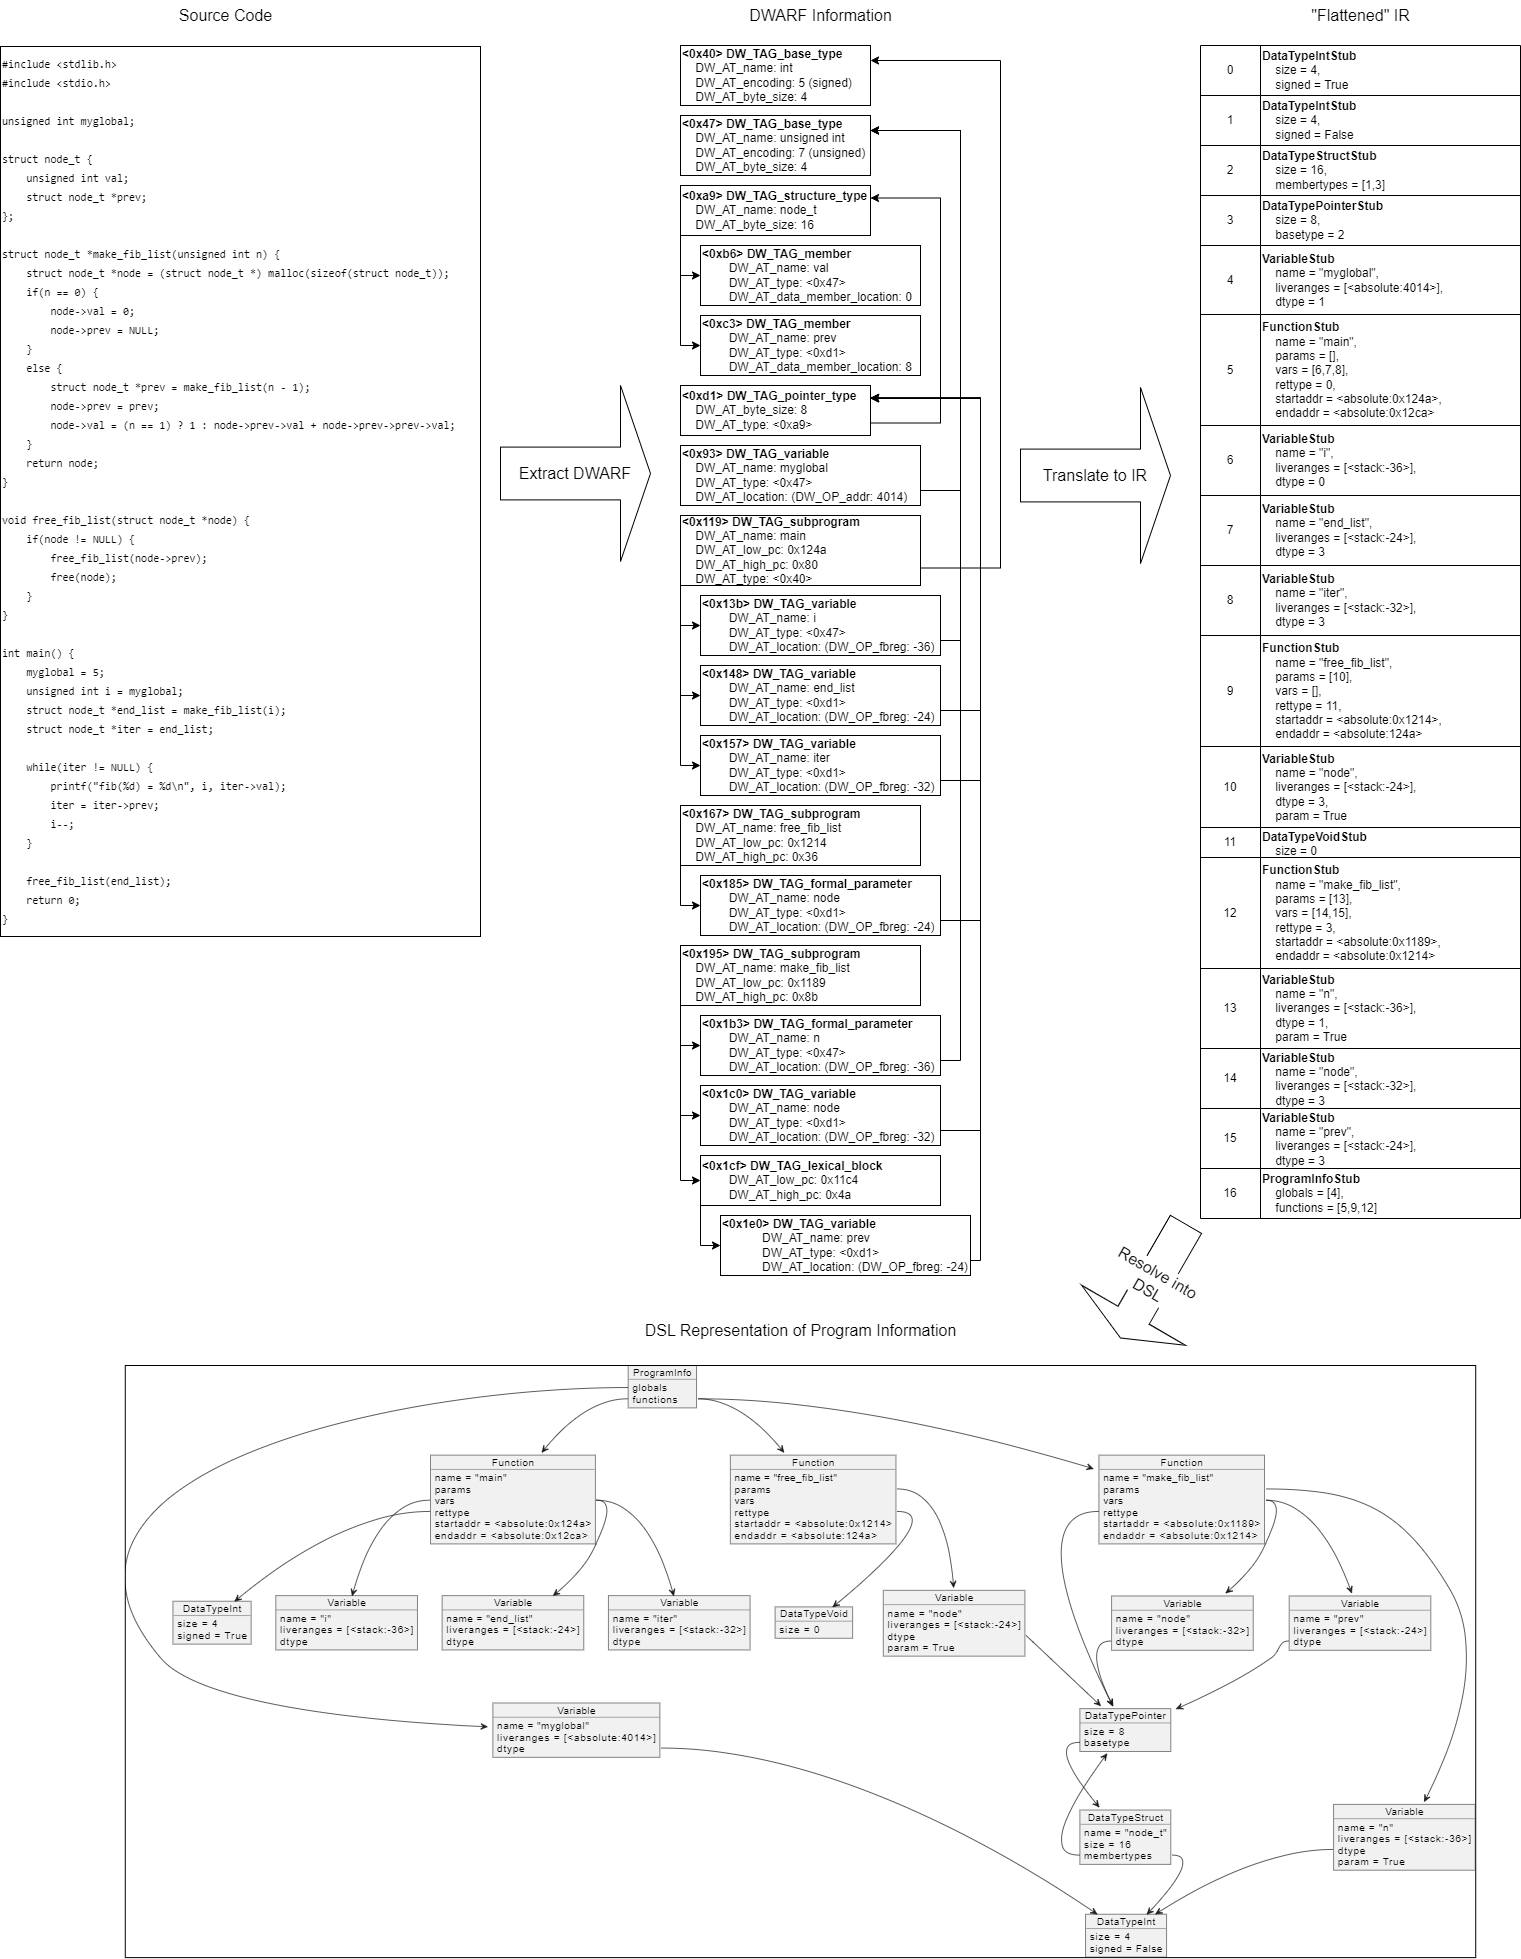
\includegraphics[width=\textwidth]{./figures/parse-dwarf.drawio.png}
    \caption{An example of translating DWARF information into the DSL}
    \label{fig:parse-dwarf}
\end{figure}

\section{Capturing Decompiler Program Information}

In addition to capturing a ground-truth program representation in our DSL, we must construct a DSL representation of the program information obtained from a decompiler we wish to evaluate. Depending on the decompiler and the structure of its output, this process may take many forms, often involving querying APIs exposed by the decompiler framework. In all cases however, this shall involve defining a translation module from the decompiler output to the structures defined in the DSL. Hence, our framework can be employed on any decompiler assuming a translation module implementation.

\subsection{Translating Ghidra Decompiler Output to the DSL}

For our analysis of the Ghidra decompiler, we utilize the Ghidra scripting API to programmatically scrape and process information about the decompilation of target binary programs. The Ghidra scripting environment exposes its own collection of data structures and functions from which we obtain our information. Since the Ghidra scripting environment supports Python, we directly import and leverage our "flattened" IR (described in the previous section) and our DSL constructs to carry out the translation.

The strategy employed for the Ghidra translation is similar to that of our DWARF translation algorithm described in the previous section. We utilize the Ghidra API to obtain particular information about functions, variables, data types, and associated addresses gathered during the decompilation. Of particular use to our translation logic is the \emph{DecompInterface} object exposed by the Ghidra API. This interface supports decompiling functions one at a time. Information inferred by each function's decompilation is used to update Ghidra's internal representation of the program information. By decompiling each of the functions extracted from Ghidra's disassembly analysis, we attempt to form a complete decompiled interpretation of the entire input program.

We use the same IR defined for the DWARF translation to accumulate flattened records corresponding to these program constructs in a database. From here, we run the same resolution algorithm on the IR constructs database to generate the root \emph{ProgramInfo} object in our DSL.

\section{Comparison of "Ground Truth" and Decompiler Program Information}

After converting both the ground-truth and decompiler program information into our DSL representation, we next formulate and implement a strategy to compare the two resulting \emph{ProgramInfo} objects. To achieve this, we create an extension of our DSL that defines data structures and functions for capturing comparison information at different layers.

\subsection{Data Type Comparison}

Given two \emph{DataType} objects and an offset between their start locations, we devise a method to capture nuanced information about the comparison of the data types.

\subsubsection{Definitions}

We define the \emph{metatype} of a data type to be general "class" of the given data type. These metatypes include \emph{INT}, \emph{FLOAT}, \emph{POINTER}, \emph{ARRAY}, \emph{STRUCT}, \emph{UNION}, \emph{UNDEFINED}, \emph{VOID}, and \emph{FUNCTION\_PROTOTYPE}. We consider \emph{INT}, \emph{FLOAT}, \emph{POINTER}, \emph{UNDEFINED}, and \emph{VOID} to be \emph{primitive metatypes} since they cannot be decomposed further. \emph{ARRAY}, \emph{STRUCT}, and \emph{UNION} are considered \emph{complex metatypes} since these types are formed via the composition or aggregation of different members or subtypes. We consider the 'char' data type to be of the \emph{INT} metatype with size equal to one byte.

% [Figure: Ariste type lattice]
\begin{figure}
    \centering
    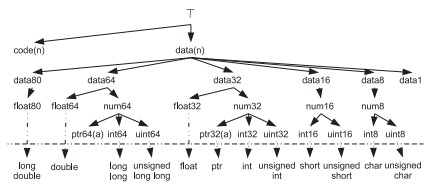
\includegraphics[width=\textwidth]{./figures/ariste-type-lattice.png}
    \caption{ARTISTE type lattice \cite{bib:artiste,bib:type-inference-executables}}
    \label{fig:artiste-type-lattice}
\end{figure}

A \emph{primitive type lattice} \cite{bib:type-inference-executables} is used to hierarchically relate primitive data types based on their metatype, size, and signedness (if applicable). More general types are located higher in the lattice while more specific types are located closer to the leaves. A type lattice may be used to determine whether two primitive data types are equivalent or share a common parent type. Our framework leverages the ARTISTE primitive type lattice defined in Caballero et. al \cite{bib:artiste} and shown in Figure \ref{fig:artiste-type-lattice}.

% [Figure: Subset relationship example(s)]

We next define a \emph{subset} relationship between two data types. For a given complex data type X and another data type Y with a given offset (possibly 0) between the location of X and Y in memory, Y is considered a \emph{subset} type of X if Y is equivalent to a "portion" of X, consistent with the offset between X and Y. For example, if X is an array, any sub-array or element of X such that elements are aligned and the element types are equivalent to X is considered a subset of X. If X is a struct or union, any sub-struct or member with proper alignment and equal constituent elements is considered a subset of X.

\subsubsection{Comparison Logic}

Suppose we have two \emph{DataType} objects X (ground truth) and Y (decompiler) with offset k from the start of X to the start of Y. The goal is to compute the \emph{data type comparison level} for the given comparison. The possible values for the comparison level are as follows, from lowest equality to highest equality:

\begin{itemize}
    \item \emph{NO\_MATCH}: No relationship could be found between X and Y.
    \item \emph{SUBSET}: Y is a subset type of the complex type X.
    \item \emph{PRIMITIVE\_COMMON\_ANCESTOR}: In the primitive type lattice, Y is an ancestor of X. This indicates that the inferred type Y is a conservative (more general) form of the ground truth type X.
    \item \emph{MATCH}: All properties of X and Y match including metatype, size, and possibly subtypes (applicable to pointers, arrays, structs, and unions).
\end{itemize}

We first check the equality of X and Y. If X and Y are equal, we assign the \emph{MATCH} comparison code. In the case that X and Y are both primitive types, we attempt to compute their shared ancestor in the primitive type lattice. If Y is an ancestor (more general form) of X, we assign \emph{PRIMITIVE\_COMMON\_ANCESTOR}. If X is a complex type, we employ an algorithm to determine whether Y is a subset of X at offset k by recursively descending into constituent portions of X starting at offset k (sub-structs, sub-arrays, elements, members) and checking for equality with Y. If a subset relationship is found, we assign the \emph{SUBSET} compare level. In all other cases, we assign the \emph{NO\_MATCH} compare level.

\subsection{Variable Comparison}

There are two main contexts where variable comparison occurs. The first context is at the top level, where the set of ground-truth global variables is compared to the set of decompiler global variables. The second context for variable comparison is within the context of a function when we compare local variables between the ground-truth and the decompiler. In either case, comparing sets of variables starts with the decomposition of each \emph{Variable} object from the DSL into a set of \emph{Varnode} objects in our extended DSL.

A \emph{Varnode} ties a \emph{Variable} to a specific storage location and the range of PC addresses indicating when variable lives at that location. The varnodes for a given variable are directly computed from the variable's live ranges discussed previously. In unoptimized binaries, it is the case that a single \emph{Variable} shall decompose into a single \emph{Varnode}.

With each variable decomposed into its associated varnodes, we next partition the varnodes from each the ground-truth and the decompiler based on the "address space" in which they reside. These address spaces include the \emph{absolute} address space, the \emph{stack} address space, and the \emph{register offset} address space (for a given register). The \emph{stack} address space is a special case of the \emph{register offset} address space where the offset register is the base pointer which points to the base of the current stack frame.

For the set of varnodes in each address space, we first order them based on their offset within the address space. Next, we attempt to find overlaps between varnodes from the two sources based on their location and size. If an overlap occurs between two varnodes, we compute a data type comparison taking into account the offset between the start locations of the two varnodes. The data type comparison approach is described in the previous section.

Based on the overlap status and data type comparison of a ground-truth varnode X, one of the following \emph{varnode comparison levels} will be assigned:

\begin{itemize}
    \item \emph{NO\_MATCH}: X is not overlapped with any varnodes from the other source.
    \item \emph{OVERLAP}: X overlaps with one or more varnodes from the other space, but the data type comparisons are level \emph{NO\_MATCH}.
    \item \emph{SUBSET}: X overlaps with one or more varnodes and each of its compared varnodes has data type comparison level equal to \emph{SUBSET}. In other words, the compared varnode(s) make up a portion of X.
    \item \emph{ALIGNED}: For some varnode Y from the other source, X and Y share the same location and size in memory; however, the data types of X and Y do not match. The data types comparison could have any comparison level less than \emph{MATCH}.
    \item \emph{MATCH}: For some varnode Y from the other source, X and Y share the same location and size in memory, and their data types match exactly.
\end{itemize}

% [Figure: Varnode comparison levels derived from varnode recovery and data type comparison]
\begin{figure}
    \centering
    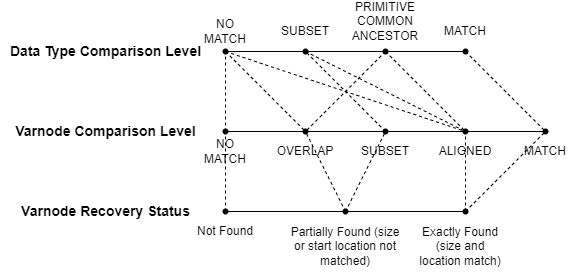
\includegraphics[width=\textwidth]{./figures/varnode-levels.drawio.png}
    \caption{Derivation of varnode comparison level from varnode recovery status and data type comparison}
    \label{fig:varnode-levels}
\end{figure}

\subsubsection{Decomposed Variable Comparison}

The inference of variables with complex data types including structs, arrays, and unions proves to be a major challenge for decompilers. Recognizing this, we develop an approach to compare the sets of ground truth and decompiler variables (varnodes) in their most "decomposed" forms. An analysis of this sort helps to recognize how well a decompiler infers the primitive constituent components of complex variables. Furthermore, this allows us to recognize the aggressiveness and accuracy of complex variable synthesis from more primitive components.

% [Figure: Example of "decomposing" complex varnode]
\begin{figure}
    \begin{subfigure}[ht]{0.25\textwidth}
        \centering
        \begin{Verbatim}[frame=single]
typedef struct {
    int day;
    int month;
    int year;
} Date;

typedef struct {
    char* name;
    int ssn;
    float height;
    float weight;
    Date dob;
} Person;

Person people[2];
        \end{Verbatim}
        \caption{Definition of a high-level variable}
        \label{fig:decompose-src}
    \end{subfigure}
    \hfill
    \begin{subfigure}[hb]{0.75\textwidth}
        \scalebox{0.35}[0.4]{\input{./figures/decompose.latex}}
        \caption{Decomposition of a high-level varnode into primitive components}
        \label{fig:decompose-tree}
    \end{subfigure}
    \caption{Example of high-level varnode decomposition}
    \label{fig:decompose}
\end{figure}

We first implement an approach to recursively strip away the "complex layers" of a varnode to its most primitive decomposition. This primitive decomposition produces a set of one or more primitive varnodes as they would appear in memory. For example, an array of elements is broken down into a set of its elements (decomposed recursively). A struct is broken down into a set of varnodes associated with each of its members (decomposed recursively). Unions present a special case since the members share a common, overlapping region of memory. Hence, to decompose a union, we transform it into an \emph{UNDEFINED} primitive type with the same size as the union.

We apply this primitive decomposition to each varnode in the sets of ground truth and decompiler varnodes. With the two sets of decomposed varnodes, we leverage the same variable comparison approach described previously to compare the varnodes in these sets. The resulting comparison information is treated as a separate analysis from the unaltered varnode sets.

% [Figure: An example of varnode comparisons on the stack]
\begin{figure}
    \centering
    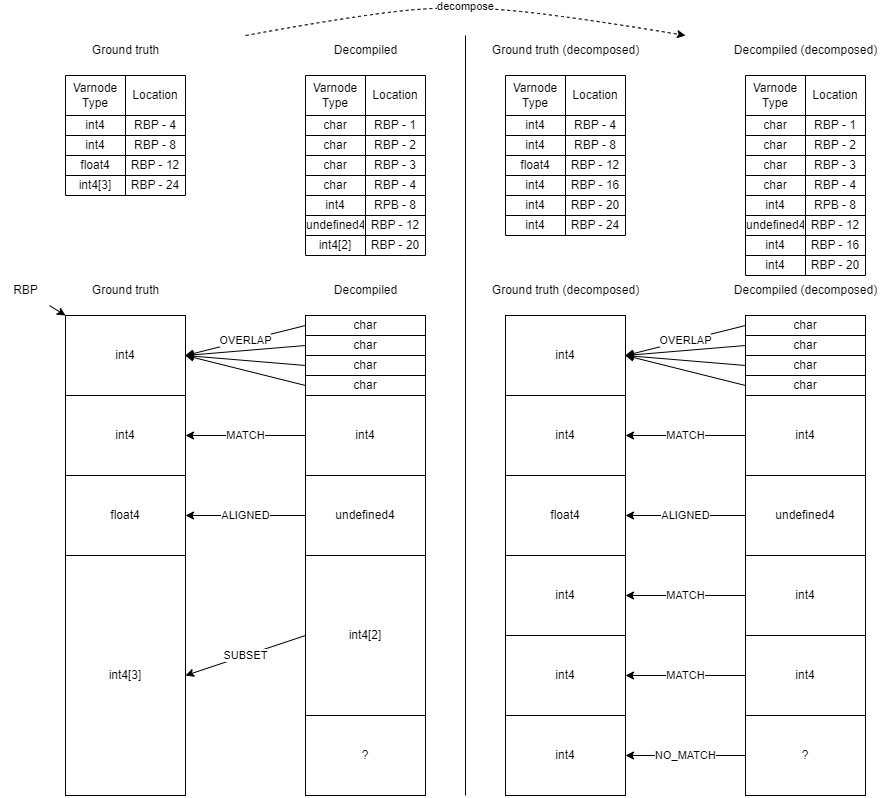
\includegraphics[width=\textwidth]{./figures/stack-comparison.drawio.png}
    \caption{An example of varnode comparisons between ground truth and decompiler varnodes for a given stack frame}
    \label{fig:stack-comparison}
\end{figure}

\subsection{Function Comparison}

The first step in function comparison is to determine whether each ground-truth function is found by the decompiler. We first order the functions from each source by the start PC address of the function. Next, we attempt to match the functions from the two sources based on start address. Any functions from the ground-truth that are not matched by a decompiler function are considered "missed". For any missed functions, we consider its associated parameters, local variables, and data types to also be "missed".

For each "matched" function based on start PC address, we compute and store information including the return type comparison, parameter comparisons, and local variable comparisons. These sub-comparisons leverage the data type and variable comparison techniques described previously.

\section{Quantitative Evaluation Metrics}

In this section, we define quantitative metrics for evaluating the accuracy of the a given decompiler when compared to a ground-truth source. We rely on the function, variable, and data type comparison information discussed previously to extract these metrics. In the following sub-sections, we define sets of metrics that associated with tables seen in Chapter \ref{sec:evaluation}.

\subsection{Functions}

This set of metrics outlines the function identification performance of the decompiler.

\begin{itemize}
    \item \emph{Ground truth functions}: The number of functions present in the ground truth program representation.
    \item \emph{Functions found}: The number of functions from the ground truth set that are identified by the decompiler.
    \item \emph{Functions missed}: The number of functions from the ground truth set that are not identified by the decompiler.
    \item \emph{Functions recovery fraction}: The fraction of ground truth functions found by the decompiler divided by the number of ground truth functions.
\end{itemize}

\subsection{Varnodes}

Recall that a \emph{Varnode} is defined to be a source-level \emph{Variable} tied to a single storage location for a range of PC addresses. In analyses of unoptimized binaries, the mapping of variables to varnodes is one to one. This set of metrics illustrates the decompiler's accuracy in recovering varnodes.

\begin{itemize}
    \item \emph{Ground truth varnodes}: The total number of varnodes present in the ground truth source. This includes varnodes associated with global and local variables from all functions.
    \item \emph{Varnodes matched @ level LEVEL}: Each ground truth varnode is associated with a \emph{varnode comparison level} (\emph{NO\_MATCH}, \emph{OVERLAP}, \emph{SUBSET}, \emph{ALIGNED}, \emph{MATCH}) during the comparison with the set of decompiler varnodes. This metric specifies the number of ground truth varnodes that are matched at the specified level.
    \item \emph{Varnodes average comparison score}: For each \emph{varnode comparison level}, we first linearly assign an integer representing the strength of the varnode comparison (\emph{NO\_MATCH} = 0, \emph{OVERLAP} = 1, \emph{SUBSET} = 2, \emph{ALIGNED} = 3, \emph{MATCH} = 4). We then normalize these scores to fall within the range zero to one. Then, for each ground truth varnode, we compute this normalized score. We take the average score over all ground truth varnodes to obtain the resulting metric. This metric approximates how well, on average, the decompiler infers the ground truth varnodes.
    \item \emph{Varnodes fraction partially recovered}: The fraction of ground truth varnodes with a match level greater than \emph{NO\_MATCH}.
    \item \emph{Varnodes fraction exactly recovered}: The fraction of ground truth varnodes with a match level equal to \emph{MATCH}.
\end{itemize}

We repeat this varnode analysis for the decomposed (primitive) set of varnodes resulting from recursively decomposing each of the high-level varnodes into its most primitive set of varnodes. We also repeat our analysis of the original set of varnodes filtered by metatype. The metatypes considered are \emph{INT}, \emph{FLOAT}, \emph{POINTER}, \emph{ARRAY}, \emph{STRUCT}, and \emph{UNION}. Lastly, we repeat the analysis of the decomposed varnodes when filtered by metatype. For this metatype analysis over the decomposed varnodes, we only consider the primitive metatypes \emph{INT}, \emph{FLOAT}, and \emph{POINTER} since the varnodes are guaranteed to be primitive.



\subsection{Data Bytes}

These metrics look at the total number of data bytes from all variables recovered by the decompiler when compared to the ground truth source.

\begin{itemize}
    \item \emph{Ground truth data bytes}: The total number of data bytes captured from the ground truth source, derived from all global and local variables.
    \item \emph{Bytes found}: The total number of data bytes recovered by the decompiler that overlap with data bytes found in the ground truth.
    \item \emph{Bytes missed}: The number of data bytes present in the ground truth that were not recovered by the decompiler.
    \item \emph{Bytes recovery fraction}: The fraction of ground truth data bytes found by the decompiler divided by the total number of ground truth bytes.
\end{itemize}

\subsection{Array Comparisons}

In this set of metrics, we aim to evaluate the accuracy of the array inference performed by the decompiler. We examine each array comparison made during the comparison of the ground truth with the decompiler and observe the discrepancies in length, size (bytes), dimensions, and element type. The following metrics are presented:

\begin{itemize}
    \item \emph{Ground truth varnodes (metatype=ARRAY)}: The number of ground truth varnodes with metatype of ARRAY.
    \item \emph{Array comparisons}: The number of array comparisons made when comparing the ground truth with the decompiler. The decompiler may infer 0 or more array varnodes for each given ground truth array varnode.
    \item \emph{Array varnodes inferred as array}: This measures how many ground truth array varnodes are compared to at least one decompiler-inferred array varnode.
    \item \emph{Array varnodes inferred as array fraction}: Equivalent to \emph{Array varnodes inferred as array} divided by \emph{Ground truth varnodes (metatype=ARRAY)}. This expresses the fraction of ground truth array varnodes that are associated with at least one decompiler array inference.
    \item \emph{Array length (elements) average error}: For each array comparison, we find the absolute difference in the number of elements inferred by the decompiler as compared to the ground truth. We then average these differences over all array comparisons to arrive at this metric.
    \item \emph{Array length (elements) average error ratio}: For each array comparison, we first find the absolute difference in the number of elements inferred by the decompiler as compared to the ground truth. We then divide this error by the length of the ground truth array to get the error as a ratio of the array size. The average of these ratios over all array comparisons produces this metric.
    \item \emph{Array size (bytes) average error}: This metric is similar to \emph{Array length (elements) average error} but measures the error in bytes instead of number of elements.
    \item \emph{Array size (bytes) average error ratio}: This metric is similar to \emph{Array length (elements) average error ratio} but computes the error in bytes instead of array elements.
    \item \emph{Array dimension match score}: This metric is the number of array comparisons where the decompiler inferred the correct number of dimensions divided by the total number of array comparisons.
    \item \emph{Array average element type comparison score}: Each \emph{data type comparison level} is first mapped to an integer as follows: \emph{NO\_MATCH} = 0, \emph{SUBSET} = 1, \emph{PRIMITIVE\_COMMON\_ANCESTOR} = 2, \emph{MATCH} = 3. We then normalize these values such that the range is scaled from 0 to 1. We refer to this as the \emph{data type comparison score}. Then, for each array comparison, we compute the \emph{data type comparison score} and subsequently average the scores across all array comparisons to generate this metric.
\end{itemize}

\chapter{Evaluation} \label{sec:evaluation}

To demonstrate our evaluation framework, we target the Ghidra decompiler (version 10.2). We use the GNU Core Utilities programs (version 9.1) as our set of benchmarks. For each of the benchmark programs, we evaluate the accuracy of Ghidra decompilation with the program compiled in three ways: (1) stripped, (2) standard (not stripped, no debugging symbols), and (3) DWARF debug symbols included. We use the results from each of these cases to discern how the amount of information included in the binary affects the Ghidra decompiler's inference accuracy. To limit the scope of our analysis, we only consider unoptimized binaries. We use the GCC compiler (version 11.1.0) to compile the benchmark programs. The architecture and operating system of the testing machine are x86-64 and Ubuntu Linux (version 20.04), respectively.

\section{Setup}

\begin{figure}
    \centering
    \scalebox{0.5}{
        \input{./figures/evaluation-process.latex}
    }
    \caption{Evaluation workflow}
    \label{fig:evaluation-process}
\end{figure}

Prior to evaluation, we compile the 105 Coreutils benchmark programs with three compilation configurations: (1) stripped, (2) standard (not stripped, no debugging symbols), and (3) DWARF debug symbols included. For each program, we first extract the ground truth information from the binary with DWARF symbols included via our DWARF translation module. We then use our Ghidra translation module to extract the Ghidra decompilation information from the binaries compiled under each of the compilation configurations. At this point, all program information from the DWARF and Ghidra sources are represented as \emph{ProgramInfo} objects in our DSL.

Next, for each program, we perform a comparison of the program information scraped from DWARF (from the "debug" binary including DWARF symbols) with the information obtained from the Ghidra decompilation of the programs under each of the compilation configurations. The information from these comparisons are expressed in the form of objects which contain comparison information about functions, variables, and data types compared between the DWARF and Ghidra sources.

With the comparisons computed for each program and compilation configuration, we use these comparisons to compute high-level metrics that summarize the performance of the Ghidra decompiler with respect to the given benchmarks and compilation configurations (stripped, standard, and debug).

\section{Function Recovery}

\begin{table}[htb]
\centering
\caption{A summary of function recovery by compilation case.}
\label{table:opts-functions-summary}
\begin{tabular}{lp{0.15\columnwidth}p{0.15\columnwidth}p{0.15\columnwidth}p{0.15\columnwidth}p{0.15\columnwidth}}
\toprule
{} &  Ground truth functions &  Functions found &  Functions missed &  Functions recovery fraction \\
\midrule
strip    &                   18139 &            18139 &                 0 &                       1.0000 \\
standard &                   18139 &            18139 &                 0 &                       1.0000 \\
debug    &                   18139 &            18135 &                 4 &                       0.9998 \\
\bottomrule
\end{tabular}
\end{table}


Tables \ref{table:functions-O0-strip}, \ref{table:functions-O0}, and \ref{table:functions-O0-debug} in the appendix present function recovery metrics of each benchmark program under the three compilation configurations. Table \ref{table:opts-functions-summary} shows the summarization of the recovery statistics accumulated over all benchmark programs. We find that over the 18139 functions present in the ground truth, the stripped and standard compilation cases produce 100\% function recovery while the debug case fails to recover four functions, resulting in a 99.9\% recovery rate. Upon examination of Table \ref{table:functions-O0-debug}, we find that all four functions missed are from the \emph{factor} program.

To determine the cause of the missed functions, we further investigate the Ghidra decompilation of \emph{factor} and find that each of the missed functions results in a decompilation error, "Low-level Error: Unsupported data-type for ResolveUnion". This indicates that an error occurred when attempting to resolve a union data type within the decompilation of these functions. Since this error only occurs in the debug compilation case, it is clear that Ghidra's parsing and interpretation of DWARF information contributes to this error. This same union data type causing the error is successfully captured and represented in our ground truth program information and, thus, this is likely a bug within Ghidra's resolution logic.

In summary, we see that Ghidra successfully finds all functions for all compilation configurations. However, in the debug case, Ghidra's attempt to interpret and utilize DWARF information to resolve a union data type in the \emph{factor} program results in a decompiler error for four functions. This error indicates a bug in Ghidra's DWARF parsing or union resolution logic.

\section{High-Level Variable (Varnode) Recovery}

To evaluate the variable (varnode) recovery accuracy of the Ghidra decompiler, we first measure the inference performance of high-level varnodes, including varnodes with complex and aggregate types such as arrays, structs, and unions. We further measure the varnode inference accuracy by metatype to decipher which of the metatypes are most and least accurately inferred by the decompiler. This analysis is performed under each compilation configuration (stripped, standard, and debug).

\begin{table*}[tb]
\centering
\caption{A summary of high-level varnode recovery by compilation case.}
\label{table:opts-varnodes-summary}
\begin{tabular}{lp{1.50cm}p{1.33cm}p{1.33cm}p{1.33cm}p{1.33cm}p{1.33cm}p{1.33cm}p{1.33cm}p{1.33cm}}
\toprule
{} & {Varnodes matched @ level NO\_MATCH} & {Varnodes matched @ level OVERLAP} & {Varnodes matched @ level SUBSET} & {Varnodes matched @ level ALIGNED} & {Varnodes matched @ level MATCH} & {Varnode comparison score} & {Varnodes fraction partially recovered} & {Varnodes fraction exactly recovered} \\
\midrule
strip    &                                               1000 &                                             1662 &                                            1001 &                                            18570 &                                          12550 &                                    0.788 &                                              0.971 &                                              0.361 \\
standard &                                                249 &                                             1450 &                                             613 &                                            19029 &                                          13442 &                                    0.816 &                                              0.993 &                                              0.386 \\
debug    &                                                 23 &                                               52 &                                              24 &                                                7 &                                          34677 &                                    0.998 &                                              0.999 &                                              0.997 \\
\bottomrule
\end{tabular}
\end{table*}


Tables \ref{table:varnodes-O0-strip}, \ref{table:varnodes-O0}, and \ref{table:varnodes-O0-debug} in the appendix show the inference of high-level varnodes for each benchmark compiled with each of the compilation configurations. This data is summarized in Table \ref{table:opts-varnodes-summary}. We find that Ghidra at least partially infers 97.2\%, 99.3\%, and 99.6\% and precisely infers 36.1\%, 38.6\%, and 99.7\% of high-level varnodes for each for the stripped, standard, and debug compilation cases, respectively. In addition, the varnode comparison scores for each compilation case are 0.788, 0.816, and 0.998, respectively. These metrics indicate that the standard compilation case slightly outperforms the stripped case in varnode inference while the debug compilation case results in significant improvements over both the stripped and standard cases, particularly in exact varnode recovery.

\begin{table*}[tb]
\centering
\caption{A summary of high-level varnode recovery by compilation case and metatype.}
\label{table:opts-varnodes-summary-metatypes}
\begin{tabular}{lp{1.50cm}p{1.50cm}p{1.33cm}p{1.33cm}p{1.33cm}p{1.33cm}p{1.33cm}p{1.33cm}p{1.33cm}}
\toprule
      &       & {Varnodes matched @ level NO\_MATCH} & {Varnodes matched @ level OVERLAP} & {Varnodes matched @ level SUBSET} & {Varnodes matched @ level ALIGNED} & {Varnodes matched @ level MATCH} & {Varnode comparison score} & {Varnodes fraction partially recovered} & {Varnodes fraction exactly recovered} \\
\midrule
\multirow{6}{*}{strip} & INT &                                                 66 &                                               48 &                                               0 &                                            12204 &                                           8681 &                                    0.850 &                                              0.997 &                                              0.413 \\
      & FLOAT &                                                  0 &                                               56 &                                               0 &                                              113 &                                             22 &                                    0.632 &                                              1.000 &                                              0.115 \\
      & POINTER &                                                 53 &                                                4 &                                               0 &                                             5834 &                                           3513 &                                    0.839 &                                              0.994 &                                              0.374 \\
      & ARRAY &                                                729 &                                              597 &                                             565 &                                               19 &                                            228 &                                    0.315 &                                              0.659 &                                              0.107 \\
      & STRUCT &                                                152 &                                              955 &                                             432 &                                              390 &                                            106 &                                    0.419 &                                              0.925 &                                              0.052 \\
      & UNION &                                                  0 &                                                2 &                                               4 &                                               10 &                                              0 &                                    0.625 &                                              1.000 &                                              0.000 \\
\cline{1-10}
\multirow{6}{*}{standard} & INT &                                                 23 &                                               48 &                                               0 &                                            12248 &                                           8680 &                                    0.851 &                                              0.999 &                                              0.413 \\
      & FLOAT &                                                  0 &                                               56 &                                               0 &                                              113 &                                             22 &                                    0.632 &                                              1.000 &                                              0.115 \\
      & POINTER &                                                 44 &                                                4 &                                               0 &                                             5836 &                                           3520 &                                    0.840 &                                              0.995 &                                              0.374 \\
      & ARRAY &                                                181 &                                              578 &                                             352 &                                               45 &                                            982 &                                    0.625 &                                              0.915 &                                              0.459 \\
      & STRUCT &                                                  1 &                                              762 &                                             257 &                                              777 &                                            238 &                                    0.560 &                                              1.000 &                                              0.117 \\
      & UNION &                                                  0 &                                                2 &                                               4 &                                               10 &                                              0 &                                    0.625 &                                              1.000 &                                              0.000 \\
\cline{1-10}
\multirow{6}{*}{debug} & INT &                                                 13 &                                               27 &                                               0 &                                                4 &                                          20955 &                                    0.998 &                                              0.999 &                                              0.998 \\
      & FLOAT &                                                  0 &                                                0 &                                               0 &                                                0 &                                            191 &                                    1.000 &                                              1.000 &                                              1.000 \\
      & POINTER &                                                  3 &                                                0 &                                               0 &                                                1 &                                           9400 &                                    1.000 &                                              1.000 &                                              1.000 \\
      & ARRAY &                                                  5 &                                               17 &                                              24 &                                                0 &                                           2092 &                                    0.986 &                                              0.998 &                                              0.978 \\
      & STRUCT &                                                  2 &                                                8 &                                               0 &                                                0 &                                           2025 &                                    0.996 &                                              0.999 &                                              0.995 \\
      & UNION &                                                  0 &                                                0 &                                               0 &                                                2 &                                             14 &                                    0.969 &                                              1.000 &                                              0.875 \\
\bottomrule
\end{tabular}
\end{table*}


In Tables \ref{table:varnodes-metatype-INT-O0-strip}-\ref{table:varnodes-metatype-UNION-O0-strip}, \ref{table:varnodes-metatype-INT-O0}-\ref{table:varnodes-metatype-UNION-O0}, and \ref{table:varnodes-metatype-INT-O0-debug}-\ref{table:varnodes-metatype-UNION-O0-debug}, we show the inference performance of high-level varnodes for each benchmark, broken down by the metatype of the ground truth varnodes, and for all compilation configurations. We summarize this information in Table \ref{table:opts-varnodes-summary-metatypes}. From the stripped and standard compilation cases, we observe that varnodes with metatype \emph{INT} are most accurately recovered when considering varnode comparison score, fraction partially recovered, and fraction exactly recovered. In the stripped case, the inference of \emph{ARRAY} varnodes shows the worst performance with a varnode comparison score of 0.315. In the standard case, varnodes with metatype \emph{STRUCT} are least accurately recovered with a varnode comparison score of 0.560, followed closely by \emph{ARRAY} and \emph{UNION}. We see that, for both the stripped and standard compilation cases, the complex (aggregate) metatypes, \emph{ARRAY}, \emph{STRUCT}, and \emph{UNION}, show the lowest recovery accuracy with respect to varnode comparison score. Among the primitive metatypes, \emph{FLOAT} shows the worst recovery metrics for these two compilation cases.

The debug compilation case demonstrates high relative recovery accuracy across varnodes of all metatypes when compared to the stripped and standard cases. Of the primitive metatypes, varnodes of the \emph{FLOAT} metatype are perfectly recovered while varnodes of the \emph{INT} and \emph{POINTER} metatypes show exact recovery percentages of 99.8\% and 99.9\%, respectively. The complex (aggregate) metatypes, on average, display slightly lower recovery metrics than the primitive metatypes in the debug compilation case. The \emph{ARRAY} metatype reveals the worst varnode comparison score at 0.986. The \emph{UNION} metatype demonstrates the lowest exact match percentage at 87.5\%.

\section{Decomposed Variable (Varnode) Recovery}

In this section, we repeat a similar varnode recovery analysis over all varnodes; however, we first recursively decompose each varnode into a set of primitive varnodes (see Section \ref{sec:methodology}). We perform this analysis over all benchmarks for each of the three compilation cases.

\begin{table*}[tb]
\centering
\caption{A summary of decomposed varnode recovery by compilation case.}
\label{table:opts-varnodes-summary-decomposed}
\begin{tabular}{lp{1.50cm}p{1.33cm}p{1.33cm}p{1.33cm}p{1.33cm}p{1.33cm}p{1.33cm}p{1.33cm}p{1.33cm}}
\toprule
{} & {Varnodes matched @ level NO\_MATCH} & {Varnodes matched @ level OVERLAP} & {Varnodes matched @ level SUBSET} & {Varnodes matched @ level ALIGNED} & {Varnodes matched @ level MATCH} & {Varnode comparison score} & {Varnodes fraction partially recovered} & {Varnodes fraction exactly recovered} \\
\midrule
strip    &                                             139776 &                                            31280 &                                               0 &                                           231267 &                                         131593 &                                    0.586 &                                              0.738 &                                              0.246 \\
standard &                                              40187 &                                            56605 &                                               0 &                                           303527 &                                         133597 &                                    0.703 &                                              0.925 &                                              0.250 \\
debug    &                                              10547 &                                              128 &                                               0 &                                                5 &                                         523236 &                                    0.980 &                                              0.980 &                                              0.980 \\
\bottomrule
\end{tabular}
\end{table*}


Similar to the high-level varnode analysis, we show the inference of the decomposed varnodes for each benchmark and for each compilation configuration in Tables \ref{table:varnodes-decomposed-O0-strip}, \ref{table:varnodes-decomposed-O0}, and \ref{table:varnodes-decomposed-O0-debug}. Table \ref{table:opts-varnodes-summary-decomposed} summarizes this information. Naturally, we expect to see lower recovery metrics compared to the high-level varnode analysis since each complex varnode is now analyzed as a set of its constituent parts. Hence, a single "missed" high-level varnode is translated into a set of primitive varnodes, each "missed" in this analysis. We find this hypothesis to hold true across all compilation cases as each the varnode comparison score, varnodes fraction partially recovered, and varnodes fraction exactly recovered show lower values than in the high-level analysis. We see that the decomposed varnode comparison scores for the strip, standard, and debug compilation cases are 0.586, 0.703, and 0.980, respectively. The varnodes fraction partially recovered are 73.8\%, 92.5\%, and 98.0\% while the varnodes fraction exactly recovered are 24.7\%, 25.0\%, and 98.0\% across the compilation cases, respectively. Interestingly, in the stripped compilation case, we find that the number of "missed" decomposed varnodes (139937) exceeds the number of "exactly matched" decomposed varnodes (131719). This is largely due to the quantity of high-level \emph{ARRAY} and \emph{STRUCT} varnodes that are missed in the stripped case.

\begin{table*}[tb]
\centering
\caption{A summary of decomposed varnode recovery by compilation case and primitive metatype.}
\label{table:opts-varnodes-summary-metatypes-decomposed}
\begin{tabular}{lp{1.50cm}p{1.50cm}p{1.33cm}p{1.33cm}p{1.33cm}p{1.33cm}p{1.33cm}p{1.33cm}p{1.33cm}}
\toprule
      &         & {Varnodes matched @ level NO\_MATCH} & {Varnodes matched @ level OVERLAP} & {Varnodes matched @ level SUBSET} & {Varnodes matched @ level ALIGNED} & {Varnodes matched @ level MATCH} & {Varnode comparison score} & {Varnodes fraction partially recovered} & {Varnodes fraction exactly recovered} \\
\midrule
\multirow{3}{*}{strip} & INT &                                             132910 &                                            28812 &                                               0 &                                           217923 &                                         125159 &                                    0.586 &                                              0.737 &                                              0.248 \\
      & FLOAT &                                                 72 &                                               73 &                                               0 &                                              103 &                                             22 &                                    0.435 &                                              0.733 &                                              0.081 \\
      & POINTER &                                               6725 &                                             2057 &                                               0 &                                            13208 &                                           6332 &                                    0.591 &                                              0.763 &                                              0.224 \\
\cline{1-10}
\multirow{3}{*}{standard} & INT &                                              40017 &                                            46846 &                                               0 &                                           290436 &                                         127505 &                                    0.707 &                                              0.921 &                                              0.253 \\
      & FLOAT &                                                  0 &                                              145 &                                               0 &                                              103 &                                             22 &                                    0.502 &                                              1.000 &                                              0.081 \\
      & POINTER &                                                132 &                                             9245 &                                               0 &                                            12955 &                                           5990 &                                    0.636 &                                              0.995 &                                              0.211 \\
\cline{1-10}
\multirow{3}{*}{debug} & INT &                                              10533 &                                              124 &                                               0 &                                                4 &                                         494143 &                                    0.979 &                                              0.979 &                                              0.979 \\
      & FLOAT &                                                  0 &                                                0 &                                               0 &                                                0 &                                            270 &                                    1.000 &                                              1.000 &                                              1.000 \\
      & POINTER &                                                 14 &                                                2 &                                               0 &                                                1 &                                          28305 &                                    0.999 &                                              1.000 &                                              0.999 \\
\bottomrule
\end{tabular}
\end{table*}


We split the decomposed varnodes by metatype and show these results in Tables \ref{table:varnodes-decomposed-metatype-INT-O0-strip}-\ref{table:varnodes-decomposed-metatype-POINTER-O0-strip}, \ref{table:varnodes-decomposed-metatype-INT-O0}-\ref{table:varnodes-decomposed-metatype-POINTER-O0}, and \ref{table:varnodes-decomposed-metatype-INT-O0-debug}-\ref{table:varnodes-decomposed-metatype-POINTER-O0-debug}. We present the summary of these results over each compilation case in Table \ref{table:opts-varnodes-summary-metatypes-decomposed}. The table shows that the stripped and standard compilation cases demostrate the poorest inference performance in terms of varnode comparison score for varnodes of metatype \emph{FLOAT}. However, we find that the percentage of "missed" \emph{INT} varnodes is worse than that of \emph{FLOAT} in the standard and debug compilation cases, and is nearly the same in the stripped case. This may be explained by the prevalence of integer (or character) arrays in the Coreutils benchmark programs when compared to other array types. Recovery accuracy of the \emph{POINTER} metatype is comparable to the \emph{INT} metatype across the three compilation cases.

\section{Data Bytes Recovery}

Following from our varnode inference analysis, we next assess the accuracy of the Ghidra decompiler with regards to the total number of data bytes recovered across all varnodes. This analysis provides an important perspective on data recovery as the size of an improperly inferred varnode may result in a wide range in the number of misinferred bytes. For example, a large array and a single character are each represented by a varnode, but the quantity of data present in the array is much greater than that of a character. Hence, it is important to capture this nuanced view of data recovery.

\begin{table}[htb]
\centering
\caption{A summary of data bytes recovery by compilation case.}
\label{table:opts-bytes-summary}
\begin{tabular}{lp{0.15\columnwidth}p{0.15\columnwidth}p{0.15\columnwidth}p{0.15\columnwidth}p{0.15\columnwidth}}
\toprule
{} &  Ground truth data bytes &  Bytes found &  Bytes missed &  Bytes recovery fraction \\
\midrule
strip    &                  1183691 &       725144 &        458547 &                    0.613 \\
standard &                  1183691 &       954105 &        229586 &                    0.806 \\
debug    &                  1183691 &      1177221 &          6470 &                    0.995 \\
\bottomrule
\end{tabular}
\end{table}


In Tables \ref{table:bytes-O0-strip}, \ref{table:bytes-O0}, and \ref{table:bytes-O0-debug}, we show the data bytes recovery metrics for each of the benchmark programs under each compilation case. We summarize the data bytes recovery for each of the compilation cases in Table \ref{table:opts-bytes-summary}. We see that Ghidra recovers 61.3\%, 80.6\%, and 99.5\% of data bytes in the stripped, standard, and debug compilation cases, respectively.

\section{Array Inference Accuracy}

The last major analysis we perform targets the array inference accuracy of the Ghidra decompiler. We aim to measure metrics regarding the total number of arrays inferred, the length and size discrepancies of compared arrays, and the similarity of element types of compared arrays. We perform this analysis across the Coreutils benchmarks and for each compilation configuration, resuling in Tables \ref{table:array-comparisons-O0-strip}, \ref{table:array-comparisons-O0}, and \ref{table:array-comparisons-O0-debug} located in the appendix. This information is summarized in Table \ref{table:opts-array-comparisons-summary}, broken down by compilation configuration.

\begin{table*}[tb]
\centering
\caption{A summary of array recovery by compilation case.}
\label{table:opts-array-comparisons-summary}
\begin{tabular}{lp{1.09cm}p{1.09cm}p{1.09cm}p{1.09cm}p{1.09cm}p{1.09cm}p{1.09cm}p{1.09cm}p{1.09cm}p{1.09cm}p{1.09cm}}
\toprule
{} & {Ground truth array varnodes} & {Array comparisons} & {Array varnodes inferred as array} & {Array varnodes inferred as array fraction} & {Array length (elements) average error} & {Array length (elements) average error ratio} & {Array size (bytes) average error} & {Array size (bytes) average error ratio} & {Array dimension match score} & {Array average element type comparison score} \\
\midrule
strip    &                                        2138 &                               823 &                                              774 &                                              0.362 &                                            134.695 &                                              2.845 &                                          458.575 &                                              0.912 &                                       0.979 &                                              0.781 \\
standard &                                        2138 &                              1579 &                                             1530 &                                              0.716 &                                            151.156 &                                              5.442 &                                          239.023 &                                              0.475 &                                       0.975 &                                              0.670 \\
debug    &                                        2138 &                              2226 &                                             2128 &                                              0.995 &                                              9.416 &                                              0.110 &                                            9.416 &                                              0.110 &                                       1.000 &                                              1.000 \\
\bottomrule
\end{tabular}
\end{table*}


Across all benchmarks, there are 2138 ground truth arrays present. For each the stripped, standard, and debug compilation cases, the number of ground truth arrays recognized as arrays by the decompiler are 774 (36.2\%), 1530 (71.6\%), and 2128 (99.5\%), respectively. We see that the numbers of array comparisons for each compilation case are greater than these metrics indicating that Ghidra infers some ground truth arrays to be more than one array.

From the array comparisons, we observe that the average absolute differential in array length (number of elements) for the stripped, standard, and debug compilation cases are 134.7, 151.2, and 9.4, respectively. When scaling these errors with respect to the length of the ground truth arrays in the comparisons, the error ratios are 2.84, 5.44, and 0.11 for the compilation cases, respectively. This reveals that, in the debug case for example, the lengths of decompiler-inferred arrays are off by an average of 9.4 elements and roughly 11\% (greater or less than) of the size of the ground truth arrays they are compared to. These metrics, however, fail to capture whether the decompiler-inferred array has element types of the correct length. Thus, a similar analysis on the size (number of bytes) errors yields errors and error ratios of 458.6 (0.91), 239 (0.47), and 9.41 (0.11) for each compilation case, respectively. This, for example, shows that arrays inferred in the standard compilation case have an average absolute byte differential of 239 and a relative error of 47\% compared to the size of the ground truth array they are compared to.

In this analysis, we also capture a measure of the array dimension match score for each compilation case. This metric measures the fraction of array comparisons where the decompiler-inferred array has the same dimensionality (one-dimensional, two-dimensional, etc.) as the ground truth array. The stripped and standard compilation cases display dimensionality match ratios of greater than 97.4\%, while the debug case shows 100\% dimensionality inference accuracy.

The last portion of our array recovery analysis focuses on the element type inference accuracy of the decompiler-inferred arrays when compared to the element types of the ground truth arrays. We compute a data type comparison score between the element types from each array comparison and average these across all array comparisons derived from our benchmark programs. This data type comparison score is similar in concept to the varnode comparison score and is described in Chapter \ref{sec:methodology}. We find that decompiler-inferred arrays in the stripped, standard, and debug compilation cases show 0.781, 0.670, and 0.999 average element type comparison scores, respectively. The better performance demonstrated in the stripped case compared to the standard case appears to be a data artifact resulting from fewer array comparisons present in the stripped analysis.

\section{Debug Compilation Case Discussion}

Upon examination of our results thus far, the reader may wonder why the debug compilation case does not produce 100\% recovery for varnodes and data bytes across all benchmarks. The same DWARF debugging information used to generate the ground truth program information is also provided to the Ghidra decompiler in this case and therefore, theoretically, Ghidra should be able to precisely capture the same program information.

We manually investigate this phenomenon over our benchmark programs and find that the cause of these recovery inaccuracies stems from the Ghidra decompiler's inflexibility in expressing local variables tied to lexical scopes. We find that the Ghidra decompiler output only lists variable declarations at the top level of the function and does not support declarations of local variables within lexical scopes. Instead, Ghidra attempts to move the declaration of these scope-specific variables to the top level of the function. Often, this behavior does not negatively influence the variable recovery of the given function. However, there are cases where multiple exclusive (not overlapping or nested) lexical scopes contain variable declarations. In many of these cases, the compiler recognizes the exclusivity of the lexical scopes and assigns the scope-specific variables to shared space on the stack since the variables shall never be instantiated simultaneously. The size of the shared region allocated by the decompiler is equivalent to the size of the largest variable in the set of scope-specific variables that share the region. In essence, this is equivalent to an implicit union formed by the compiler. The DWARF debugging standard and our DSL both possess the ability to express these overlapping scope-specific variables, but the Ghidra decompiler does not. From our observations, we find that Ghidra greedily captures and declares scope-specific variables at the top level of the function based on the order in which it recovers the variables. In the debug compilation case (utilizing DWARF information), Ghidra appears to only consider the first scope-specific variable mapped to a given address on the stack based on the order of the variables in the list of debugging information entries (DIEs) parsed from DWARF. The subsequent scope-specific variables associated with the given address are simply ignored, causing Ghidra to potentially miss several varnodes and data bytes. We consider this to be a shortcoming and an area of future improvement for the Ghidra decompiler.

% [Figure: Ghidra missing variable in 2nd scope]
\begin{figure}
    \centering
    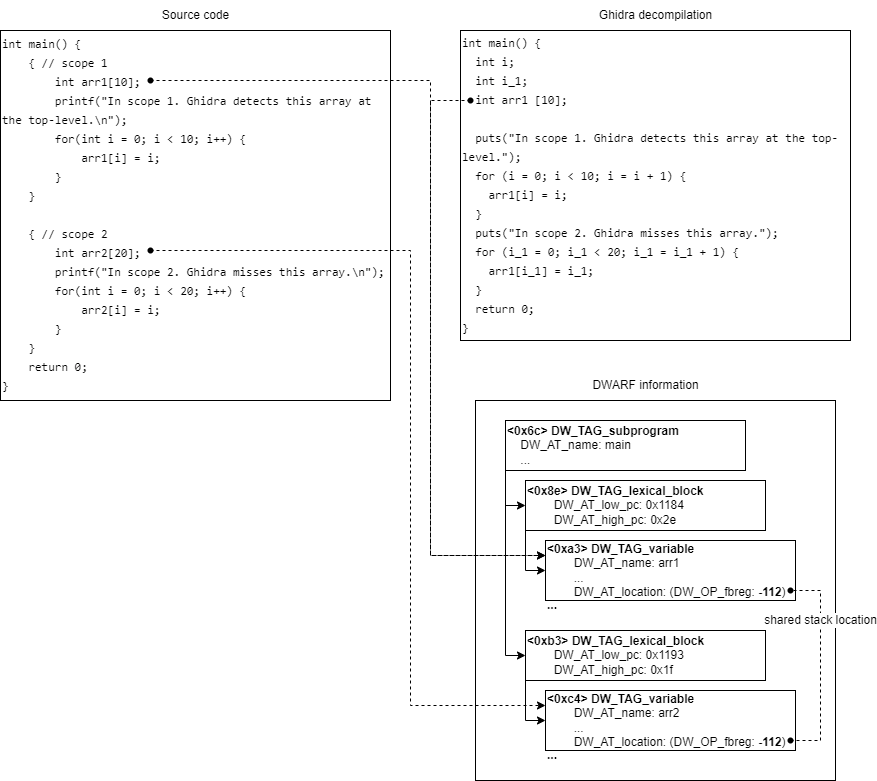
\includegraphics[width=\textwidth]{./figures/ghidra-miss-scopes.drawio.png}
    \caption{An example of the Ghidra decompiler missing the second of two scope-specific variables that share stack space}
    \label{fig:ghidra-miss-scopes}
\end{figure}

\chapter{Conclusion} \label{sec:conclusion}

\section{Summary of Methodology}

To develop our decompiler evaluation framework, we outline and execute the following objectives:

\begin{enumerate}
    \item Express program information such as functions, variables, data types, and addresses in a common representation.
    \item Programmatically capture a "ground truth" representation for a given program.
    \item Programmatically scrape program information from decompiler tools, namely Ghidra.
    \item Compare two program representations of the same program.
    \item Formulate quantitative metrics for evaluating the accuracy of a decompiler.
\end{enumerate}

We devise and implement a common domain-specific language (DSL) for expressing the association of high-level program information such as functions, variables, and data types, with binary-level constructs such as addresses and storage locations. With our DSL, we develop a parser for extracting DWARF debugging information from binary programs and representing this information in our DSL. This information is to be used as a ground truth source of program information in comparisons with decompiler representations. Next, we leverage the Ghidra Python API to develop a translator module, taking Ghidra decompilation output as our input and translating the information into our DSL. With our parsing modules constructed for both our ground truth and decompiler soures, we extend our DSL to support the comparison of two sources of program information parsed from a ground truth source and a decompiler source. We subsequently develop quantitative metrics for assessing and summarizing comparisons of program information sources.

\section{Summary of Results}

We utilize our developed framework to assess the recovery performance of the Ghidra decompiler (version 10.2) over the 105 GNU Core Utilities (version 9.1) benchmark programs. Using the GCC compiler (version 11.1.0), we compile the benchmarks with no optimizations under three separate compilation configurations: (1) stripped, (2) standard (not stripped, no DWARF symbols added), (3) debug (DWARF symbols included).

Our function recovery analysis reveals that Ghidra recovers 100\% of the 18139 functions across all benchmarks in the stripped and standard compilation cases. In the debug case, we find four missed functions in total, all present in the \emph{factor} benchmark program. We discover that the missed functions are all caused by a decompiler error resulting from a failure in resolving a union data type. We conclude that this is a bug in the Ghidra decompiler.

In our high-level varnode analysis, we find that the recovery accuracy of primitive (\emph{INT}, \emph{FLOAT}, \emph{POINTER}) metatypes is greater than that of the complex (aggregate) metatypes (\emph{ARRAY}, \emph{STRUCT}, \emph{UNION}) across all compilation cases. This finding follows from the fact that inferring complex varnodes involves an extra layer of speculation and inference involving the synthesis of low-level varnodes. In all compilation cases, the \emph{ARRAY} metatype displays the greatest number of "missed" varnodes.

Our decomposed (primitive) varnode analysis demonstrates that Ghidra is least effective at inferring floating-point (metatype \emph{FLOAT}) decomposed varnodes over the benchmark programs in the stripped and standard compilation cases. However, we see that Ghidra completely misses a larger fraction of decomposed varnodes with metatype \emph{INT}. This is explained by the larger incidence of integer arrays in the Coreutils benchmark programs, which are more likely to be missed or only partially recovered as demonstrated in our high-level varnode analysis. We show that decomposed varnodes of metatype \emph{POINTER} are recovered comparably to those of metatype \emph{INT}.

In our analysis of data bytes recovery summarized across all benchmarks, we find that the Ghidra decompiler shows 61.3\% recovery in the stripped compilation case, 80.6\% recovery in the standard case, and 99.5\% recovery in the debug case.

Our array inference analysis illustrates that the compilation configuration of our benchmark programs has a significant impact on both array recovery and the inference accuracy of the arrays that are recovered. We find that, for each the stripped, standard, and debug compilation cases, 36.2\%, 71.6\%, and 99.5\% of ground truth array varnodes overlap with at least one associated decompiler-inferred array varnode, respectively. We find the average size error ratio of the decompiler-inferred arrays with respect to the ground truth arrays to be 0.91, 0.47, and 0.11 for the compilation cases, respectively.

The function, variable, data bytes, and data type recovery analyses show clear recovery accuracy differentials between the three compilation cases. In general, we find that the debug case (DWARF symbols included) performs the best by a large margin, followed by the standard case which slightly outperforms the stripped case. Despite the decent recovery performance in the debug case, we seek an explanation for the decompiler still failing to capture a portion of the ground truth information, particularly varnodes and data bytes. We find that the Ghidra decompiler is limited in its ability to express overlapping stack variables gathered from disjoint (non-overlapping, non-nested) lexical scopes within the same parent function. This scenario arises when the compiler recoginizes the exclusivity of lexical scopes within a function and subsequently assigns scope-specific variables from these lexical scopes to the same address or region on the stack.

\section{Limitations}

The primary limitation of our framework in its current state is the lack of support for comparing and evaluating program information gathered from optimized binary programs. Our DSL supports the expression of program information from optimized binaries, but the comparison logic assumes certain properties about the program information to reduce the complexity of the analysis. Future work shall include the extension of the framework to support the evaluation of optimized binaries.

Another assumption in our analysis is that only non-parameter variables with stack and absolute (global) addresses are considered for comparison. Heap-allocated data must be referenced by a local or global pointer and therefore heap data recovery evaluation is performed indirectly via this pointer. Application of existing static analysis techniques are necessary to peform a more complete evaluation of heap constructs.

Another limitation in this work is our exclusive support for the DWARF debugging standard for extracting ground truth program information. However, as discussed previously, our framework can easily be extended to support the implementation of parsers for other debugging formats.

Regarding decompiler evaluation, our framework excels at assessing the recovery and inference of high-level program constructs. However, our framework lacks the ability to evaluate behavioral correctness and overall clarity of decompiler output. Existing works, including those by Liu et al. \cite{bib:how-far-weve-come} and Naeem et al. \cite{bib:metrics-effectiveness-decompilers}, have proposed strategies for assessing these aspects. A comprehensive decompiler evaluation shall combine our structural recovery analysis with these forms of analyses.

The final noteworthy limitation in our work is that we use our framework to assess only the Ghidra decompiler. We consider our framework to be the primary contribution of this research and therefore leave the analysis and comparison of other decompilers for future work.

\section{Future Work}

As discussed in the previous section, a major future work objective shall be to extend our framework to support optimized binaries. Another area for improvement shall be to include existing static analysis techniques to identify and more accurately assess the recovery of heap-allocated data. Lastly, we shall use our framework to assess and compare the recovery performance of decompilers beyond Ghidra.

In our function recovery analysis, recall that the Ghidra decompiler fails to decompile four functions within the \emph{factor} program only in the case where DWARF debugging symbols are included. We conclude from the error messages returned that the decompilation errors for these functions result from Ghidra's inability to resolve a particular union data type present in the program. Since this error does not occur for the other compilation cases of the \emph{factor} program, we gather that the DWARF information scraped by Ghidra contributes to this error. With this observation, we recognize that a useful obfuscation strategy for binary programs may, instead of stripping all debugging symbols, be to include misleading and contradictory debugging information. Reverse engineering tools and decompilers analyzing a binary program with misleading debugging symbols included may produce incorrect outputs or potentially crash based on this erroneous information. This is certainly an area worthy of future research. In addition, the union resolution issue observed in our analysis shall be patched in the Ghidra framework.

In our assessment of the Ghidra decompiler, we observe that Ghidra does not successfully capture all ground truth variables and data bytes even in the case the DWARF debugging information is present. Upon further investigation, we discover this shortcoming is due to Ghidra's inability to express local variable declarations at lexical scope levels below the top level of a function. In other words, Ghidra forces all local variables to be declared at the top level of a given function. This causes Ghidra to partially miss cases where the same stack address region is used by the compiler to store local variables declared in non-overlapping, non-nested lexical scopes within the same function. An direction for future work shall be to modify the Ghidra decompiler to support the expression of more flexible local variable constructs that are not required to be declared at the top level of a function.

% Bibliography, default style from former template.
\nocite{*}
\global\long\def\bibname{References}
\bibliography{references}

\chapter*{Appendix}
\appendix
\small

% functions - stripped
\input{data/tables/functions-O0-strip.tex}
% functions - standard
\input{data/tables/functions-O0.tex}
% functions - debug
\input{data/tables/functions-O0-debug.tex}


% varnodes - stripped
\input{data/tables/varnodes-O0-strip.tex}

% varnodes - stripped - INT
\input{data/tables/varnodes-metatype-INT-O0-strip.tex}
% varnodes - stripped - FLOAT
\input{data/tables/varnodes-metatype-FLOAT-O0-strip.tex}
% varnodes - stripped - POINTER
\input{data/tables/varnodes-metatype-POINTER-O0-strip.tex}
% varnodes - stripped - ARRAY
\input{data/tables/varnodes-metatype-ARRAY-O0-strip.tex}
% varnodes - stripped - STRUCT
\input{data/tables/varnodes-metatype-STRUCT-O0-strip.tex}
% varnodes - stripped - UNION
\input{data/tables/varnodes-metatype-UNION-O0-strip.tex}


% varnodes - standard
\input{data/tables/varnodes-O0.tex}

% varnodes - standard - INT
\input{data/tables/varnodes-metatype-INT-O0.tex}
% varnodes - standard - FLOAT
\input{data/tables/varnodes-metatype-FLOAT-O0.tex}
% varnodes - standard - POINTER
\input{data/tables/varnodes-metatype-POINTER-O0.tex}
% varnodes - standard - ARRAY
\input{data/tables/varnodes-metatype-ARRAY-O0.tex}
% varnodes - standard - STRUCT
\input{data/tables/varnodes-metatype-STRUCT-O0.tex}
% varnodes - standard - UNION
\input{data/tables/varnodes-metatype-UNION-O0.tex}


% varnodes - debug
\input{data/tables/varnodes-O0-debug.tex}

% varnodes - debug - INT
\input{data/tables/varnodes-metatype-INT-O0-debug.tex}
% varnodes - debug - FLOAT
\input{data/tables/varnodes-metatype-FLOAT-O0-debug.tex}
% varnodes - debug - POINTER
\input{data/tables/varnodes-metatype-POINTER-O0-debug.tex}
% varnodes - debug - ARRAY
\input{data/tables/varnodes-metatype-ARRAY-O0-debug.tex}
% varnodes - debug - STRUCT
\input{data/tables/varnodes-metatype-STRUCT-O0-debug.tex}
% varnodes - debug - UNION
\input{data/tables/varnodes-metatype-UNION-O0-debug.tex}


% decomposed varnodes - stripped
\input{data/tables/varnodes-decomposed-O0-strip.tex}

% decomposed varnodes - stripped - INT
\input{data/tables/varnodes-decomposed-metatype-INT-O0-strip.tex}
% decomposed varnodes - stripped - FLOAT
\input{data/tables/varnodes-decomposed-metatype-FLOAT-O0-strip.tex}
% decomposed varnodes - stripped - POINTER
\input{data/tables/varnodes-decomposed-metatype-POINTER-O0-strip.tex}


% decomposed varnodes - standard
\input{data/tables/varnodes-decomposed-O0.tex}

% decomposed varnodes - standard - INT
\input{data/tables/varnodes-decomposed-metatype-INT-O0.tex}
% decomposed varnodes - standard - FLOAT
\input{data/tables/varnodes-decomposed-metatype-FLOAT-O0.tex}
% decomposed varnodes - standard - POINTER
\input{data/tables/varnodes-decomposed-metatype-POINTER-O0.tex}


% decomposed varnodes - debug
\input{data/tables/varnodes-decomposed-O0-debug.tex}

% decomposed varnodes - debug - INT
\input{data/tables/varnodes-decomposed-metatype-INT-O0-debug.tex}
% decomposed varnodes - debug - FLOAT
\input{data/tables/varnodes-decomposed-metatype-FLOAT-O0-debug.tex}
% decomposed varnodes - debug - POINTER
\input{data/tables/varnodes-decomposed-metatype-POINTER-O0-debug.tex}


% data bytes - stripped
\input{data/tables/bytes-O0-strip.tex}
% data bytes - standard
\input{data/tables/bytes-O0.tex}
% data bytes - debug
\input{data/tables/bytes-O0-debug.tex}

% array comparisons - stripped
\input{data/tables/array-comparisons-O0-strip.tex}
% array comparisons - standard
\input{data/tables/array-comparisons-O0.tex}
% array comparisons - debug
\input{data/tables/array-comparisons-O0-debug.tex}

\end{document}